\begin{savequote}[45mm]
\ascii{Any fool can write code that a computer can understand. Good programmers write code that humans can understand.}
\qauthor{\ascii{- Martin Flower}}
\end{savequote}

\chapter{算法骨架} 
\label{ch:skeleton}

\begin{content}

\end{content}

\section{前置}

\begin{content}

一般地,在执行测试前需要预置\ascii{setUp}实施测试环境的初始化工作,完成资源的准备。对既有的用例实施重构。

\subsection{测试用例}

\begin{diff}{test/mars/core/TestCaseSpec.cc}
 \begin{c++}
#include <gtest/gtest.h>
#include "mars/core/TestCase.h"

namespace {
  struct SimpleTest : TestCase {
    bool wasRun = false;

  private:
    void run() override {
      wasRun = true;
    }
  };

  void run(TestCase& test) {
    test.run();
  }
}

TEST(SimpleTest, make_sure_test_case_can_run_normally) {
  SimpleTest test;
  run(test);

  ASSERT_TRUE(test.wasRun);
}

TEST(SimpleTest, make_sure_test_case_can_run_normally) {
  SimpleTest test;
  run(test);

  ASSERT_TRUE(test.wasRun);
}

TEST(SimpleTest, make_sure_test_case_can_run_normally) {
  SimpleTest test;
  run(test);

  ASSERT_TRUE(test.wasRun);
}

TEST(SimpleTest, make_sure_test_case_can_run_normally) {
  SimpleTest test;
  run(test);

  ASSERT_TRUE(test.wasRun);
}
 \end{c++}
\tcblower
 \begin{c++}
#include <gtest/gtest.h>
#include "mars/core/TestCase.h"

namespace {
  struct SimpleTest : TestCase {
    bool wasSetUp = false;
    bool wasRun = false;

  private:
    void setUp() override {
      wasSetUp = true;
    }

    void runTest() override {
      wasRun = true;
    }
  };
}

TEST(SimpleTest, make_sure_test_case_can_run_normally) {
  SimpleTest test;
  test.run();

  ASSERT_TRUE(test.wasSetUp);
  ASSERT_TRUE(test.wasRun);
}
 \end{c++} 
\end{diff}

被覆写的\ascii{SimpleTest::setUp, SimpleTest::runTest}成员函数被显式声明为\ascii{override}与\ascii{private}。前者在编译时完成函数签名的合法性检查,后者限制外部用户使用\ascii{SimpleTest}对象直接调用\ascii{setUp, runTest}成员函数。

\begin{episode}{private与override}
\begin{content}

\subsubsection{按接口编程}

一般地,在面向对象程序设计中,需要遵循“按接口类型编程”的基本设计原则。在\ascii{C++}设计语言中,接口(或抽象基类)使用虚函数声明抽象函数,子类使用\ascii{override}覆写虚函数。在编译时,编译期按照抽象的接口类型确定函数调用关系;在运行时,根据对象的具体类型在相应的虚表中检索对应的成员函数,完成运行时多态的调用。

因此,除非存在特殊的需求,将\ascii{override}函数\ascii{private}化,以明确对外声明:在编译时,无法通过该具体类型实现对\ascii{override}函数的直接调用;推荐使用抽象的接口类型或基类型,在运行时实现多态调用。

\subsubsection{例外}

凡事都存在例外,被覆写的析构函数就不应该声明为\ascii{private};否则,无法生成该类型的值对象,因为没办法析构。

\end{content}
\end{episode}

\subsection{通过编译}

重构\ascii{TestCase},仅公开\ascii{run}方法,并移除运行时多态的特性,它负责组织用例执行运行时的算法骨架。搬迁运行时多态行为至私有的两个虚函数,用户根据自己的场景定制\ascii{setUp}与\ascii{runTest},分别完成测试准备,及其测试执行。

\begin{leftbar}
 \begin{c++}[caption={\ttfamily{include/mars/core/TestCase.h}}]
struct TestCase {
  virtual ~TestCase() {}

  void run();

private:
  virtual void setUp() {}
  virtual void runTest() {}
};
  \end{c++}
\end{leftbar}

\begin{episode}{善用快捷键}
\begin{content}

\subsubsection{场景1}

在\ascii{C++}编程实践中,需要经常在头文件、实现文件、测试文件中频繁切换;而且头文件声明的成员函数,需要在实现文件中实现。幸运的是,\ascii{Eclipse IDE}提供了相关快捷键,让这些事情变得不再麻烦。

\begin{enum}
  \eitem{\code{Ctrl + Tab}: 在头文件与实现文件之间切换;}
  \eitem{\code{Ctrl + E}: 打开最近打开的文件列表;}  
  \eitem{\code{Alt + Shift + S}: 实现头文件中声明的函数;}      
  \eitem{\code{Ctrl + Shift + N}: 自动导入缺失的头文件。}      
\end{enum}

\subsubsection{场景2}

“重命名函数”是最常见的一种重构手法,如果严格遵循重构过程,需要每个步骤都谨小慎微。

\begin{enum}
  \eitem{新建一个函数;}
  \eitem{拷贝旧函数的实现至新函数;}
  \eitem{编译,测试通过;}
  \eitem{删除旧函数的实现逻辑,转调新函数;}
  \eitem{编译,测试通过;}
  \eitem{对于每个引用旧函数的地方,重构引用新函数,确保编译、测试通过;}    
  \eitem{删除旧函数。}      
\end{enum}

\ascii{Eclipse IDE}提供了重命名类与函数的快捷键\ascii{Alt + Shift + R},轻松搞定这件事情。善用快捷键,不仅可以提高编程的效率,也能提高重构的安全性。

\subsubsection{快捷键}

没有必要掌握所有的快捷键,但需要熟悉常用的快捷键。在结对编程实践中,向同伴学习,或推荐同伴,都是一件极其有意思的事情。

\begin{enum}
  \eitem{大杀器}
\begin{enum}
  \eitem{\code{Ctrl + Shift + L}: 列出所有的快捷键,恢复记忆;}
\end{enum}

  \eitem{导航类}
\begin{enum}
  \eitem{\code{Ctrl + Shift + R}: 跳转到特定文件,常使用模糊匹配方式搜索文件;}
  \eitem{\code{Ctrl + Shift + T}: 跳转至某个符号,例如类,函数,全局变量;}
  \eitem{\code{Alt + } $\leftarrow/\rightarrow$: 跳转至上一个/下一个编辑点;} 
  \eitem{\code{Ctrl + E}: 在最近打开的文件列表中切换;}
  \eitem{\code{Ctrl + O}: 在当前文件中的函数之间切换;}
  \eitem{\code{Ctrl + Q}: 跳转到最后编辑过的位置;}  
  \eitem{\code{Ctrl + L}: 跳转至特定的行,定位编译错误很有用;}
  \eitem{\code{Ctrl + =}: 宏展开;}        
  \eitem{\code{Ctrl + T}: 查看继承层次;}
  \eitem{\code{Alt + Shift + S}: 代码生成视图;}
  \eitem{\code{Alt + Shift + N}: 新建文件视图;}
\end{enum}

  \eitem{光标类}
\begin{enum}
  \eitem{\code{Ctrl + }$\leftarrow/\rightarrow$: 逐单词向左/向右移动光标;}
  \eitem{\code{Shift + }$\leftarrow/\rightarrow$: 逐字符向左/向右选择;}
  \eitem{\code{Ctrl + Shift + }$\leftarrow/\rightarrow$: 逐单词向左/向右选择;}
  \eitem{\code{Shift + Home/End}: 从当前光标选择至行首/行末;}  
  \eitem{\code{Shift + }$\downarrow/\uparrow$: 选择当前行/上一行;}  
  \eitem{\code{Ctrl + Shift + }$\downarrow/\uparrow$: 移动光标至下一个/上一个成员;}    
  \eitem{\code{Ctrl + A}: 全选;}  
\end{enum}
      
  \eitem{编辑类}
\begin{enum}
  \eitem{\code{Ctrl + D}: 删除当前行;}
  \eitem{\code{Alt + }$\uparrow/\downarrow$: 向上/向下移动当前行;}   
  \eitem{\code{Ctrl + Alt + }$\uparrow/\downarrow$: 向上/向下复制当前行;}     
  \eitem{\code{Ctrl + Shift + F}: 格式化;}
  \eitem{\code{Ctrl + Shift + N}: 自动导入缺失的头文件;}  
  \eitem{\code{Ctrl + Shift + X/Y}: 转为小写/大写;} 
  \eitem{\code{Alt + Shift + A}: 列模式}
  \eitem{\code{Alt + Shift + R}: 重命名;}
  \eitem{\code{Ctrl + Alt + J}: 合并行;}  
  \eitem{\code{Ctrl + Z}: 撤销;}
  \eitem{\code{Ctrl + Shift + Z}: 恢复;}      
\end{enum}

  \eitem{功能键}
\begin{enum}
  \eitem{\code{F2}: 重命名文件名;}
  \eitem{\code{F3}: 跳转类、函数定义;}
  \eitem{\code{F4}: 查看继承层次;}  
\end{enum}

  \eitem{注释类}
\begin{enum}
  \eitem{\code{Ctrl + }$/$: 单行注释,或取消单行注释;} 
  \eitem{\code{Ctrl + shift +  }$/$: 多行注释;} 
  \eitem{\code{Ctrl + shift +  } $\backslash$: 取消多行注释;}   
\end{enum}

  \eitem{查找类}
\begin{enum}
  \eitem{\code{Ctrl + H}: 打开搜索对话框;} 
  \eitem{\code{Ctrl + K}: 在文件内查找下一个该符号的位置;} 
  \eitem{\code{Ctrl + Shift + K}: 在文件内查找上一个该符号的位置;}   
  \eitem{\code{Ctrl + shift + G}: 查找该符号所有的引用;} 
  \eitem{\code{Ctrl + shift + H}: 查看函数的调用关系;}   
\end{enum}

\end{enum}

\end{content}
\end{episode}

\subsection{通过测试}

实现\ascii{TestCase::run}的主体逻辑。

\begin{leftbar}
 \begin{c++}[caption={\ttfamily{src/mars/core/TestCase.cc}}]
#include "mars/core/TestCase.h"

void TestCase::run() {
  setUp();
  runTest();
}
 \end{c++}
\end{leftbar}

测试通过。

\end{content}

\section{后置}

\begin{content}

\subsection{测试用例}

同理,测试执行后使用\ascii{tearDown}完成现场清理,释放资源。用户通过定制私有的虚函数\ascii{tearDown}完成此功能。

\begin{leftbar}
 \begin{c++}[caption={\ttfamily{test/mars/core/TestCaseSpec.cc}}]
#include <gtest/gtest.h>
#include "mars/core/TestCase.h"

namespace {
  struct SimpleTest : TestCase {
    bool wasSetUp = false;
    bool wasRun = false;
    bool wasTearDown = false;

  private:
    void setUp() override {
      wasSetUp = true;
    }

    void runTest() override {
      wasRun = true;
    }

    void tearDown() override {
      wasTearDown = true;
    }
  };
}

TEST(SimpleTest, make_sure_test_case_can_run_normally) {
  SimpleTest test;
  test.run();

  ASSERT_TRUE(test.wasSetUp);
  ASSERT_TRUE(test.wasRun);
  ASSERT_TRUE(test.wasTearDown);  
}
 \end{c++}
\end{leftbar}

\begin{episode}{struct与class}
\begin{content}

关键字\ascii{struct}是\cpp{}继承自\clang{}的一项遗产。作为更加贴切的词汇,\ascii{class}被引入\cpp{},用来表示\emph{类}。但是,\cpp{}增强了\ascii{struct}既有的语义,赋予了\ascii{class}同等的超能力。这样的决策引入了一个选择的难题:如何明确地界定\ascii{struct}与\ascii{class}使用的标准呢?

这个问题在社区内也并无定论,甚至\cpp{}的发明者\ascii{Bjarne Stroustrup}也无法给出明确的建议。在语法层上,\ascii{struct}和\ascii{class}的差异体现在\emph{默认可见性}:\ascii{struct}默认为\ascii{public},而\ascii{class}则为\ascii{private}。表面上,两者仅存在语法层面的外在差异性,实则存在价值观的潜在差异性。

\subsubsection{误区}

社区常遵循这样一个规则:使用\ascii{struct}定义数据,不应该定义行为;否则,就使用\ascii{class}定义类。表面看似合理,实则是一个误区。

当然,如果使用\cpp{}开发一个库,并提供一套可供\clang{}语言调用的接口,这个规定是合理的。如果不是基于此类目的,这个规则便是自找麻烦。因为一个类型是否应该定义行为,是随软件演进过程而动态变化的。最初定义的时候,可能以持有数据为主要目的,但无法确保随后不会因为某种目的而为其添加一个方法,简单举例说明。

存在一个结构体\ascii{Rectangle}表示矩形,这是一个纯数据的结构体。

\begin{c++}
struct Rectangle {
  int width;
  int height;
};
\end{c++}

随后,发现客户代码出现大量重复设计。

\begin{c++}
Rectangle r;

r.width = 2;
r.heigth = 4;

bool area = r.width * r.height;
\end{c++}

为了消除重复,可以提取一个初始化函数。

\begin{c++}
void init_rectangle(Rectangle* r, int width, int height) {
  r->width = width;
  r->width = height;
}

int get_area_rectangle(Rectangle* r) {
  return r->width * r->height;
}
\end{c++}

客户如此方式使用这两个\ascii{API}。

\begin{c++}
Rectangle r;
init_rectangle(&r, 2, 4);

int area = get_area_rectangle(&r);
\end{c++}

这是\clang{}语言典型的实现方法。殊途同归,老练的\ascii{C++}程序员,会将其搬迁至成员函数。

\begin{c++}
struct Rectangle {
  Rectangle(int width, int height) : width(width), height(height) {
  }

  int getArea() const {
    return width * height;
  }

  int width;
  int height;
};
\end{c++}

这种做法不仅没有引入任何额外的内存和性能开销。甚至,由于使用了初始化列表,它的性能还略微得到改善。除此之外,还收获了一些其它好处。

\begin{enum}
  \eitem{增强了内聚性:数据与行为在同一个类域内;} 
  \eitem{增强了安全性: 避免对象不经意地发生未初始化的错误;} 
  \eitem{增强了可理解性:客户代码更加的简洁,直观。} 
\end{enum}

而遵循上述规则,则需要将\ascii{Rectangle}修正使用\ascii{class}。但是,这需要在所有的客户代码中,将前置声明\ascii{struct Rectangle}修正为\ascii{class Rectangle};否则,编译期将提示告警信息。显然,这个规则不能支持软件设计的长期演进的需求。

以这种原则来区分使用\ascii{struct},还是\ascii{class},不会带来任何好处,相反只会带来一堆麻烦。于是,不难得出这样的结论:只应该坚持使用其中一个。问题归结于:到底是哪个更好呢?

\subsubsection{接口定义时的差异}

\begin{c++}
class Runnable {
public:
  virtual void run() = 0;
  virtual ~Runnable() {}
};

struct Runnable {
  virtual void run() = 0;
  virtual ~Runnable() {}
};
\end{c++}

两者差别甚微,但却体现了不同的价值观。对于一个纯虚类,从逻辑上本来就是一个只有公开方法声明,没有实现细节的接口类型。在这样的契约关系下,再通过\ascii{public}指明其公开性,纯属画蛇添足。

懒惰的我讨厌冗余,讨厌重复。更何况从平衡和美感的角度看,那个横立的\ascii{public}犹如洁白墙面上的一沫蚊子血,显得格外刺眼。

\subsubsection{继承时的差异}

\begin{c++}
class TestCase : public TestFixture, public Test {
  // ...
};

struct TestCase : TestFixture, Test {
  // ...  
};
\end{c++}

在\ascii{C++}编程实践中,至少$90\%$的情况都会使用公有继承。这就意味着,如果在绝大多数情况下,都要重复地指明\ascii{public},显然不是一个理性的选择。

\subsubsection{类定义的差异}

\[\text{程序} = \text{数据结构} + \text{算法}\]

\begin{c++}
class TestCase : public TestFixture, public Test {
  std::string name;

public:
  explicit TestCase(const std::string& name);
};

struct TestCase : TestFixture, Test {
  explicit TestCase(const std::string& name);

private:
  std::string name;
};
\end{c++}

对于把程序理解为“数据结构+算法”的程序员,尽管正在使用面向对象的元素——“类”,却依然会认为理解一个程序的前提是理解它的数据结构。在这样的价值观驱动下,把私有数据摆在前面就是完全合情合理的。数年前,我就曾在一本C++相关的书中读到过这样的建议。

但对于越来越确信信息隐藏对软件之重要的我,则更倾向于认为公开接口才是了解一个模块最关键的知识。当试图去使用一个模块时,我总是会优先查看它的测试用例(如果有的话),然后再去看它的公开接口声明。一般而言,这对于理解它能做什么,以及如何使用它已经足够;接口声明处的私有元素反而会干扰我对一个模块的理解。只有在好奇心的驱使下,我才会进一步去看看它的实现。

基于这样的认知,当定义一个类的时候,我会把公开方法定义在前面。至于私有的内容,我总是会竭尽所能的不希望引起人们的注意,宁愿付出一些代价,也要把它们藏到别人在类声明里看不到的地方,更不会放在前面扰乱视听。

\subsubsection{一致性}

\end{content}
\end{episode}

\subsection{通过编译}

当用例执行完成后,\ascii{TestCase::tearDown}负责清理现场。

\begin{leftbar}
 \begin{c++}[caption={\ttfamily{include/mars/core/TestCase.h}}]
struct TestCase {
  virtual ~TestCase() {}

  void run();

private:
  virtual void setUp() {}
  virtual void runTest() {}
  virtual void tearDown() {}
};
  \end{c++}
\end{leftbar}

\subsection{通过测试}

至此,完成了运行一个用例的主干逻辑,但缺乏异常处理机制,留待后续处理。

\begin{leftbar}
 \begin{c++}[caption={\ttfamily{src/mars/core/TestCase.cc}}]
#include "mars/core/TestCase.h"

void TestCase::run() {
  setUp();
  runTest();
  tearDown();
}
 \end{c++}
\end{leftbar}

\end{content}

\section{算法骨架}

\begin{content}

\ascii{TestCase::run}实现了\ascii{xUnit}最核心的高层算法逻辑,实现了高层算法逻辑与底层实现细节的解耦,并且实现了高层算法逻辑的高度复用。如\refig{simple-test}所示。

\begin{figure}[H]
\centering
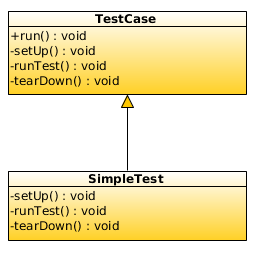
\includegraphics[width=0.4\textwidth]{figures/xunit/simple-test.png}
\caption{模板方法:定义算法骨架}
 \label{fig:simple-test}
\end{figure}

\subsection{引入策略}

模板方法模式与策略模式都可以用来分离高层的算法与具体的实现细节。之前已经看到了模板方法的实现,接下来探讨策略模式实现的效果,并从中对比两者之间的差异,从而指导设计的权衡与取舍。

\subsubsection{测试用例}

\ascii{TestCaseRunner}构建高层算法逻辑,而\ascii{TestCase}作为\ascii{TestCaseRunner}的抽象策略。新增测试用时,覆写\ascii{TestCase}相关接口,完成具体实现细节。实现\ascii{TestCaseRunner}的高层算法逻辑与\ascii{SimpleTest}的具体实现细节之间关系的解耦。

\begin{leftbar}
 \begin{c++}
namespace {
  struct SimpleTest : TestCase {
    bool wasSetUp = false;
    bool wasRun = false;
    bool wasTearDown = false;

  private:
    void setUp() override {
      wasSetUp = true;
    }

    void runTest() override {
      wasRun = true;
    }

    void tearDown() override {
      wasTearDown = true;
    }
  };
}

TEST(SimpleTest, run_test_case_using_strategry) {
  SimpleTest test;
  TestRunner runner(test);
  runner.run();

  ASSERT_TRUE(test.wasSetUp);
  ASSERT_TRUE(test.wasRun);
  ASSERT_TRUE(test.wasTearDown);  
}
 \end{c++}
\end{leftbar}

\subsubsection{通过测试}

\ascii{TestRunner::run}负责组织高层算法逻辑,算法子步骤的实现通过抽象的\ascii{TestCase}委托给某个具体策略对象完成。从而实现了\ascii{TestCaseRunner}与\ascii{SimpleTest}之间的解耦,两者都依赖于抽象的\ascii{TestCase},如\refig{simple-test-strategry}所示。

\begin{figure}[H]
\centering
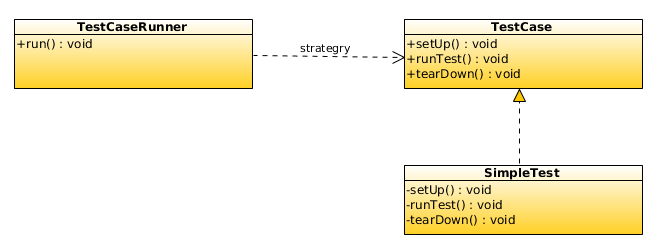
\includegraphics[width=1.0\textwidth]{figures/xunit/simple-test-strategry.png}
\caption{策略对象:定义算法骨架}
 \label{fig:simple-test-strategry}
\end{figure}


\begin{leftbar}
 \begin{c++}
struct TestCase {
  virtual ~TestCase() {}

  virtual void setUp() {}
  virtual void runTest() {}
  virtual void tearDown() {}
};

struct TestCaseRunner {
  TestCaseRunner(TestCase& test) : test(test) {
  }

  void run() {
    test.setUp();
    test.runTest();
    test.tearDown();
  }

private:
  TestCase& test;
};
 \end{c++}
\end{leftbar}

\subsection{权衡利弊}

使用模板方法,\ascii{SimpleTest}通过继承方式直接复用了\ascii{TestCase::run}高层算法逻辑。但继承是一种强依赖,增强了\ascii{SimpleTest}与\ascii{TestCase}之间的耦合关系。

使用策略方法,\ascii{TestCaseRunner}高层算法逻辑与\ascii{SimpleTest}是解耦的,但额外地引入类\ascii{TestCaseRunner}。

既然两个方案都有优缺点,到底应该采用哪个方案呢?其一,使用策略方法,需要建立额外的委托关系,不仅增加过多的类,使得设计变得更加复杂。其二,观察\ascii{TestCaseRunner::run}的实现,其实现基本完全委托给了\ascii{TestCase};按照迪米特法则,这段高层算法逻辑应该归属于\ascii{TeseCase}。

\begin{leftbar}
\begin{c++}
void TestCaseRunner::run() {
  test.setUp();
  test.runTest();
  test.tearDown();
}
\end{c++}
\end{leftbar}

按照这个推理,实施重构将\ascii{TestCaseRunner::run}搬迁至\ascii{TestCase},\ascii{TestCaseRunner}就成为一个空类,根本就没有存在的理由。因此,按照迪米特法则,也应优选模板方法。

如果优选模板方法,那么需要分析一下此场景使用模板方法的带来的副作用。无非就是因为引入继承关系从而增强了\ascii{TestCase}与\ascii{SimpleTest}的耦合关系。但是,考虑到\ascii{SimpleTest}是\ascii{xUnit Mars}最小调度单位,不会进一步被继承或组合而被复用,这个耦合关系仅局部于\ascii{SimpleTest}内部,不会被传播到其他地方,这是完全可以接受的设计。



\end{content}
